% Fibonacci spiral
% Author: Andrew Mertz
\documentclass{standalone}
\usepackage{amsmath,tikz}
\usepackage{xfp}
\usepackage[lite,subscriptcorrection,slantedGreek,nofontinfo]{mtpro2}
\newcommand{\num}[1]{\langle\mathbf{#1}\rangle\hspace*{1em}}
\newcommand{\name}[1]{\langle\mathbf{#1}\rangle}

\usetikzlibrary{positioning}
%% helper macros

% The 3D code is based on The drawing is based on Tomas M. Trzeciak's 
% `Stereographic and cylindrical map projections example`: 
% http://www.texample.net/tikz/examples/map-projections/
\newcommand\pgfmathsinandcos[3]{%
  \pgfmathsetmacro#1{sin(#3)}%
  \pgfmathsetmacro#2{cos(#3)}%
}
\newcommand\LongitudePlane[3][current plane]{%     
  \pgfmathsinandcos\sinEl\cosEl{#2} % elevation
  \pgfmathsinandcos\sint\cost{#3} % azimuth
  \tikzset{#1/.estyle={cm={\cost,\sint*\sinEl,0,\cosEl,(0,0)}}}
}
\newcommand\LatitudePlane[3][current plane]{%
  \pgfmathsinandcos\sinEl\cosEl{#2} % elevation
  \pgfmathsinandcos\sint\cost{#3} % latitude
  \pgfmathsetmacro\yshift{\cosEl*\sint}
  \tikzset{#1/.estyle={cm={\cost,0,0,\cost*\sinEl,(0,\yshift)}}} %
}
\newcommand\DrawLongitudeCircle[2][1]{
  \LongitudePlane{\angEl}{#2}
  \tikzset{current plane/.prefix style={scale=#1}}
   % angle of "visibility"
  \pgfmathsetmacro\angVis{atan(sin(#2)*cos(\angEl)/sin(\angEl))} %
  \draw[current plane,thin,white] (\angVis:1) arc (\angVis:\angVis+180:1);
  \draw[current plane,thin,white,dashed] (\angVis-180:1) arc (\angVis-180:\angVis:1);
}%this is fake: for drawing the grid
\newcommand\DrawLongitudeCirclered[2][1]{
  \LongitudePlane{\angEl}{#2}
  \tikzset{current plane/.prefix style={scale=#1}}
   % angle of "visibility"
  \pgfmathsetmacro\angVis{atan(sin(#2)*cos(\angEl)/sin(\angEl))} %
  \draw[current plane,white] (150:1) arc (150:180:1);
  %\draw[current plane,dashed] (-50:1) arc (-50:-35:1);
}%for drawing the grid
\newcommand\DLongredd[2][1]{
  \LongitudePlane{\angEl}{#2}
  \tikzset{current plane/.prefix style={scale=#1}}
   % angle of "visibility"
  \pgfmathsetmacro\angVis{atan(sin(#2)*cos(\angEl)/sin(\angEl))} %
  \draw[current plane,white,dashed] (150:1) arc (150:180:1);
}
\newcommand\DLatred[2][1]{
  \LatitudePlane{\angEl}{#2}
  \tikzset{current plane/.prefix style={scale=#1}}
  \pgfmathsetmacro\sinVis{sin(#2)/cos(#2)*sin(\angEl)/cos(\angEl)}
  % angle of "visibility"
  \pgfmathsetmacro\angVis{asin(min(1,max(\sinVis,-1)))}
  \draw[current plane,white,dashed] (-50:1) arc (-50:-35:1);

}
\newcommand\fillred[2][1]{
  \LongitudePlane{\angEl}{#2}
  \tikzset{current plane/.prefix style={scale=#1}}
   % angle of "visibility"
  \pgfmathsetmacro\angVis{atan(sin(#2)*cos(\angEl)/sin(\angEl))} %
  \draw[current plane,white,thin] (\angVis:1) arc (\angVis:\angVis+180:1);

}

\newcommand\DrawLatitudeCircle[2][1]{
  \LatitudePlane{\angEl}{#2}
  \tikzset{current plane/.prefix style={scale=#1}}
  \pgfmathsetmacro\sinVis{sin(#2)/cos(#2)*sin(\angEl)/cos(\angEl)}
  % angle of "visibility"
  \pgfmathsetmacro\angVis{asin(min(1,max(\sinVis,-1)))}
  \draw[current plane,thin,white] (\angVis:1) arc (\angVis:-\angVis-180:1);
  \draw[current plane,thin,white,dashed] (180-\angVis:1) arc (180-\angVis:\angVis:1);
}%Defining functions to draw limited latitude circles (for the red mesh)
\newcommand\DrawLatitudeCirclered[2][1]{
  \LatitudePlane{\angEl}{#2}
  \tikzset{current plane/.prefix style={scale=#1}}
  \pgfmathsetmacro\sinVis{sin(#2)/cos(#2)*sin(\angEl)/cos(\angEl)}
  % angle of "visibility"
  \pgfmathsetmacro\angVis{asin(min(1,max(\sinVis,-1)))}
  %\draw[current plane,red,thick] (-\angVis-50:1) arc (-\angVis-50:-\angVis-20:1);
\draw[current plane,white] (-50:1) arc (-50:-35:1);

}

\tikzset{%
  >=latex,
  inner sep=0pt,%
  outer sep=2pt,%
  mark coordinate/.style={inner sep=0pt,outer sep=0pt,minimum size=3pt,
    fill=white,circle}%
}
\usepackage{amsmath}
\usetikzlibrary{arrows}
\pagestyle{empty}
\usepackage{pgfplots}
\usetikzlibrary{calc,fadings,decorations.pathreplacing}

\newcommand{\im}[2][3.5]{%
    \lower-.2em\hbox{
    \scalebox{#1}[#1]{%
    \ensuremath{\displaystyle #2}%
}}}

\usetikzlibrary{backgrounds,calc}
\begin{document}
% I have seen many beautiful depictions of Fibonacci spirals and
% golden spirals. So I thought it would be nice to make a Fibonacci
% spiral in TikZ. I like the look of white on black so here I define a
% black background rectangle.
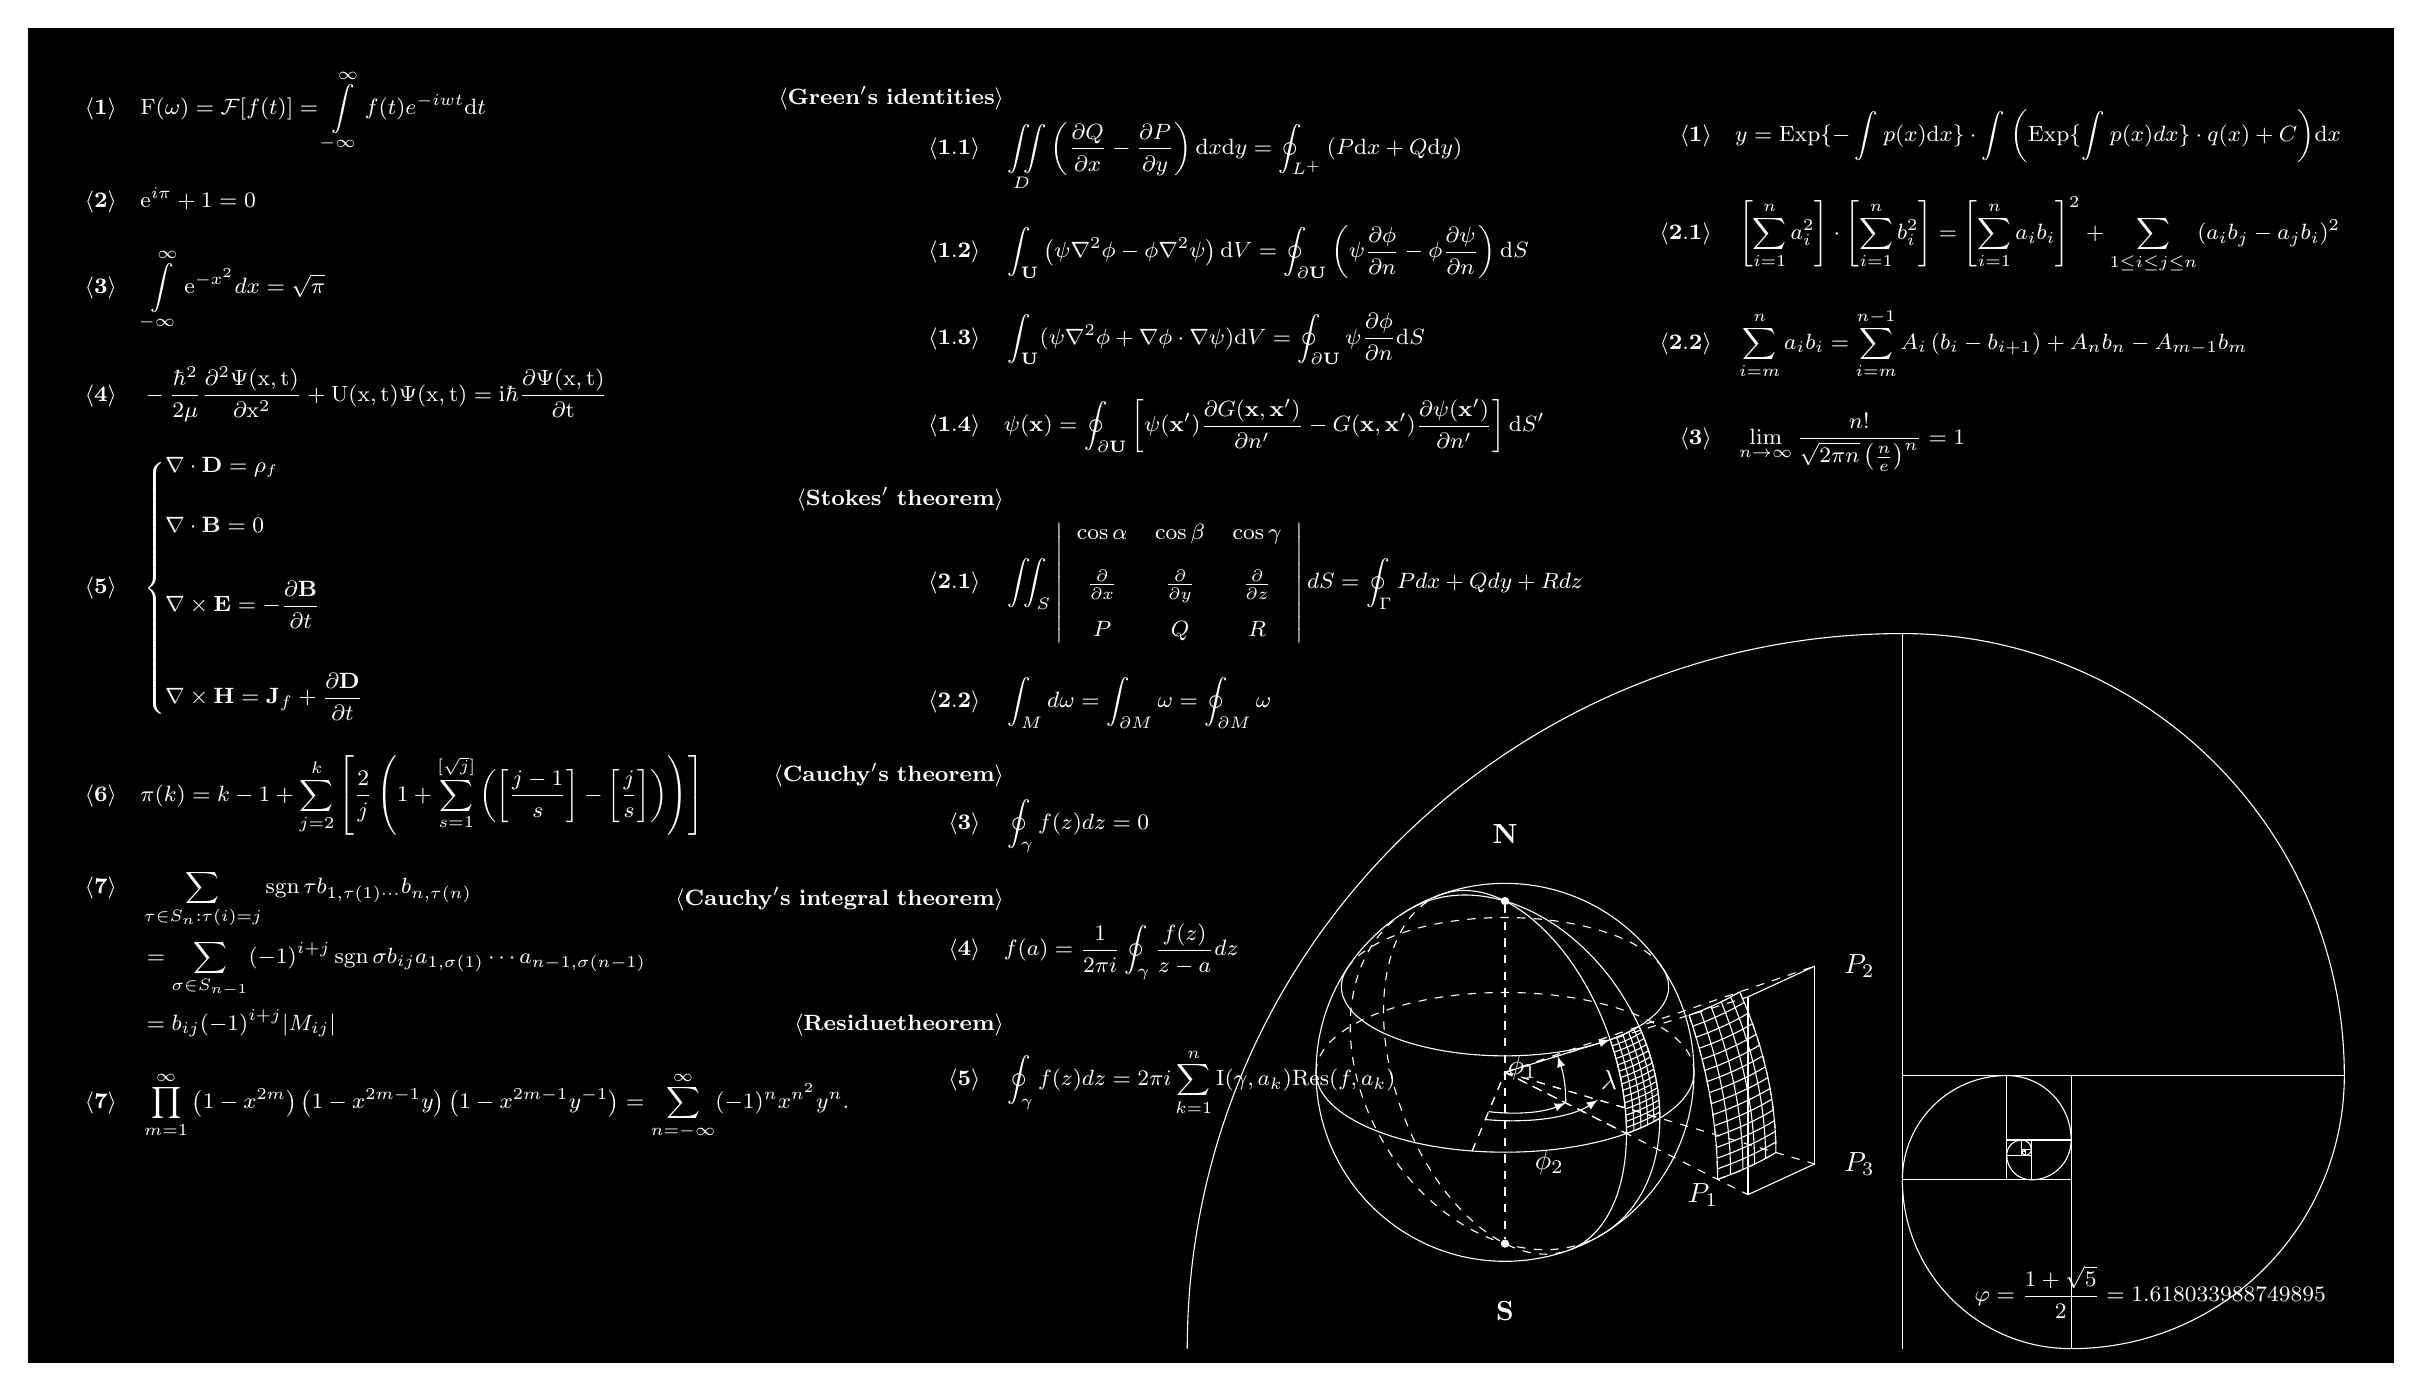
\begin{tikzpicture}[background rectangle/.style={fill=black},
                    show background rectangle] 
  % Create some counters for holding the Fibonacci numbers
  \newcounter{a}
  \newcounter{b}
  \newcounter{temp}

  % Initialize the counters
  \setcounter{a}{0}
  \setcounter{b}{1}

  % The spiral will start at the origin
  \coordinate (0) at (0,0);

  % This loop defines the number of turns in the spiral. Note that we
  % will have to be careful not to overflow our counters or make the
  % spiral too large for TeX to handle. This is easy to do as the
  % Fibonacci sequence grows exponentially.
  \foreach \i in {1,...,18}
  {
    % Get the "name" of the last point on the spiral
    \pgfmathsetmacro{\lastpoint}{\i-1}

    % Compute the angle for this turn of the spiral
    \pgfmathsetmacro{\startangle}{mod(\i-1,4) * 90}

    % Draw this turn of the spiral and remember the point where we end 
    \draw[white] (\lastpoint) arc 
      (\startangle : \startangle + 90 : \value{b}/10.0pt) coordinate (\i);

   % Compute the next Fibonacci number
    \setcounter{temp}{\value{b}}
    \addtocounter{b}{\value{a}}
    \setcounter{a}{\value{temp}}
 }

 % Add some framing for the spiral while at the same time not "boxing"
 % it in. Note that to put a square around each turn of the spiral we
 % could have just used the command \draw[white] (\lastpoint)
 % rectangle (\i); after drawing each turn in the loop above.
 \foreach \i in {1,3,...,17}
 {
   \pgfmathsetmacro{\lastpoint}{\i-1}
   \draw[white] (\lastpoint) -| (\i);
 }

 \foreach \i in {2,4,...,16}
 {
   \pgfmathsetmacro{\lastpoint}{\i-1}
   \draw[white] (\lastpoint) |- (\i);
 }

 \draw[white] (17) -- (17 |- 18);
 \node at ($(18) + (15,9)$) {\hspace*{1em}};
 
 % Add some text displaying the formula for the Fibonacci numbers
 \node(eq) at ($(18) + (11,.7)$) 
   [white,text width = 2cm,font=\fontsize{8}{8}\selectfont] {
   \begin{displaymath}
		{\varphi} = \frac{1+\sqrt{5}}{2} = \fpeval{(1+sqrt(5))/2}
   \end{displaymath}
  };
  
   \node at ($(18) + (-14.4,9)$) {\hspace*{1em}};
   \node(eq) at ($(18) + (-13,9)$) 
   [white,text width = 2cm,font=\fontsize{8}{8}\selectfont] {
   \begin{align*}
		\num{1}& \mathrm{F}(\omega)=\mathcal F[f(t)]=\int\limits_{-\infty}^\infty f(t)e^{-iwt}\mathrm{d}t\\[1em]
		\num{2}& \mathrm{e}^{i\pi}+1=0\\[1em]
		\num{3}& \int\limits_{-\infty}^{\infty}\mathrm{e}^{-x^2}dx=\sqrt{\pi}\\[1em]
		\num{4}& -\frac{\hbar^2}{2\mu}\frac{\partial^2\Psi(\mathrm x,\mathrm t)}{\partial \mathrm x^2}+\mathrm U(\mathrm x,		\mathrm t)\Psi(\mathrm x,\mathrm t)=\mathrm i\hbar\frac{\partial\Psi(\mathrm x,\mathrm t)}{\partial\mathrm t}\\[1em]
		\num{5}& \left\{
		\begin{aligned}
			& \nabla\cdot\mathbf D=\rho_{\scriptscriptstyle f}\\ \\ 
			& \nabla\cdot\mathbf B=0\\ \\ 
			& \nabla\times\mathbf E=-\dfrac{\partial\mathbf B}{\partial t}\\ \\ 
			& \nabla\times\mathbf H=\mathbf J_f+\dfrac{\partial\mathbf D}{\partial t}
		\end{aligned}
		\right.\\[1em]
		\num{6}& \pi(k)=k-1+\sum_{j=2}^{k}\left[\frac{2}{j}\left(1+\sum_{s=1}^{[\sqrt{j}]}%
		\left(\left[\frac{j-1}{s}\right]-\left[\frac{j}{s}\right]\right)\right)\right]\\[1em]
		\num{7}& \sum\limits_{\tau\in S_n:\tau(i)=j}\operatorname{sgn}\tau b_{1,\tau(1)\cdots} b_{n,\tau(n)}\\
		& =\sum_{\sigma\in S_{n-1}}(-1)^{i+j}\operatorname{sgn}\sigma b_{ij}a_{1,\sigma(1)}\cdots a_{n-1,\sigma(n-1)} \\
		& =b_{i j}(-1)^{i+j}|M_{i j}|\\[1em]
		\num{7}&\prod_{m=1}^{\infty}\left(1-x^{2m}\right)\left(1-x^{2m-1}y\right)\left(1-x^{2m-1}y^{-1}\right)=\sum_{n=-\infty}^{\infty}(-1)^nx^{n^2}y^n.\\[1em]
   \end{align*}
  };
  
   \node(eq) at ($(18) + (-5.5,9.5)$) 
   [white,text width = 2cm,font=\fontsize{8}{8}\selectfont] {
   \begin{align*}
   		\name{Green's\ identities}&\\
		\num{1.1} & \iint\limits_D\left(\dfrac{\partial Q}{\partial x}-\dfrac{\partial P}{\partial y}\right)
		\mathrm{d}x\mathrm{d}y=\oint_{L^{+}}\left(P\mathrm{d}x+Q\mathrm{d}y\right)\\[1em]
		\num{1.2}& \int_{\mathbf{U}}\left(\psi\nabla^2\phi-\phi\nabla^2\psi\right)\mathrm{d}V=\oint_{\partial\mathbf{U}}\left(\psi\dfrac{\partial\phi}{\partial n}-\phi\dfrac{\partial\psi}{\partial n}\right)\mathrm{d}S\\[1em]
		\num{1.3}& \int_{\mathbf{U}}(\psi\nabla^2\phi+\nabla\phi\cdot\nabla\psi)\mathrm{d}V
		  =\oint_{\partial\mathbf{U}}\psi\dfrac{\partial\phi}{\partial n}\mathrm{d}S\\[1em]
		\num{1.4} & \psi(\mathbf{x})=\oint_{\partial\mathbf{U}}\left[\psi(\mathbf{x}')\dfrac{\partial G(\mathbf{x},\mathbf{x}')}{\partial n'}-G(\mathbf{x},\mathbf{x}')\dfrac{\partial\psi(\mathbf{x}')}{\partial n'}\right]\mathrm{d}S'\\[1em]
		\name{Stokes'\ theorem}&\\
		\num{2.1}& \iint_S\left|\begin{array}{ccc}
			\cos\alpha&\cos\beta&\cos\gamma\\[1em]
			\frac{\partial}{\partial x}
			&\frac{\partial}{\partial y}&\frac{\partial}	{\partial z}\\[1em] 
			P&Q&R
		\end{array}
		\right|dS=\oint_\Gamma P dx+Qdy+Rdz\\[1em]
		\num{2.2}& \int_M d\omega=\int_{\partial M}\omega=\oint_{\partial M}\omega \\[1em]
		\name{Cauchy's\ theorem}\\
		\num{3} & \oint_\gamma f(z)dz=0\\[1em]
		\name{Cauchy's\ integral\ theorem}&\\
		\num{4} & f(a)=\dfrac{1}{2\pi i}\oint_\gamma\dfrac{f(z)}{z-a}dz\\[1em]
		\name{Residue theorem}&\\
		\num{5}&\oint_\gamma f(z)dz=2\pi i\sum_{k=1}^n\mathrm I(\gamma,a_k)\mathrm{Res}(f,a_k)
   \end{align*}
  };
  
  
 \node(eq) at ($(18) + (7,13)$) 
   [white,text width = 2cm,font=\fontsize{8}{8}\selectfont] {
   \begin{align*}
		\num{1}&  y=\mathrm{Exp}\{{-\int_{}^{}{p(x){\rm d}x}}\}\cdot
		\int_{}^{}{\biggl(\mathrm{Exp}\{{\int_{}^{}{p(x) {d\rm }x}}\} \cdot q(x)+C\biggr) {\rm d}x}\\[1em]
		\num{2.1}& \left[\sum_{i=1}^{n}{a_i^2}\right]\cdot \left[\sum_{i=1}^{n}{b_i^2}\right]
        =\left[\sum_{i=1}^{n}{a_ib_i}\right]^2 + \sum_{1\le i \le j \le n}({a_ib_j-a_jb_i})^2\\[1em]
		\num{2.2} & \sum\limits_{i=m}^{n}a_ib_i=\sum\limits_{i=m}^{n-1}A_i\left(b_i-b_{i+1}\right)+A_nb_n-A_{m-1}b_m\\[1em]
		\num{3} & \lim\limits_{n\to\infty}\dfrac{n!}{\sqrt{2\pi n}\left(\frac{n}{e}\right)^n}=1\\[1em]
   \end{align*}
  };
  
\begin{scope}[shift={(-6.6, 1)},scale=.6,every node/.style={minimum size=1cm}]
	%% some definitions
	
	\def\R{4} % sphere radius
	
	\def\angEl{25} % elevation angle
	\def\angAz{-100} % azimuth angle
	\def\angPhiOne{-50} % longitude of point P
	\def\angPhiTwo{-35} % longitude of point Q
	\def\angBeta{30} % latitude of point P and Q
	
	%% working planes
	
	\pgfmathsetmacro\H{\R*cos(\angEl)} % distance to north pole
	\LongitudePlane[xzplane]{\angEl}{\angAz}
	\LongitudePlane[pzplane]{\angEl}{\angPhiOne}
	\LongitudePlane[qzplane]{\angEl}{\angPhiTwo}
	\LatitudePlane[equator]{\angEl}{0}
	% \fill[ball color=white!10] (0,0) circle (\R); % 3D lighting effect
	\draw[color=white] (0,0) circle (\R);
	\coordinate (O) at (0,0);
	\coordinate[mark coordinate] (N) at (0,\H);
	\coordinate[mark coordinate] (S) at (0,-\H);
	\path[xzplane] (\R,0) coordinate (XE);
	
    %defining points outsided the area bounded by the sphere
	\path[qzplane] (\angBeta:\R+5.2376) coordinate (XEd);
	\path[pzplane] (\angBeta:\R) coordinate (P);%fino alla sfera
	\path[pzplane] (\angBeta:\R+5.2376) coordinate (Pd);%sfora di una quantità pari a 10 dopo la sfera
	\path[pzplane] (\angBeta:\R+5.2376) coordinate (Td);%sfora di una quantità pari a 10 dopo la sfera
	\path[pzplane] (\R,0) coordinate (PE);
    \path[pzplane] (\R+4,0) coordinate (PEd);
	\path[qzplane] (\angBeta:\R) coordinate (Q);
	\path[qzplane] (\angBeta:\R) coordinate (Qd);%sfora di una quantità pari a 10 dopo la sfera
	
	\path[qzplane] (\R,0) coordinate (QE);
    \path[qzplane] (\R+4,0) coordinate (QEd);%sfora di una quantità 10 dalla sfera sul piano equat.


    \DrawLongitudeCircle[\R]{\angPhiOne} % pzplane
    \DrawLongitudeCircle[\R]{\angPhiTwo} % qzplane
    \DrawLatitudeCircle[\R]{\angBeta}
    \DrawLatitudeCircle[\R]{0} % equator
	%labelling north and south
	\node[above=8pt, white] at (N) {$\mathbf{N}$};
	\node[below=8pt, white] at (S) {$\mathbf{S}$};
	
	\draw[-,dashed, white,thin] (N) -- (S);
	\draw[->,white] (O) -- (P);
	\draw[dashed,white] (XE) -- (O) -- (PE);
	\draw[dashed,white] (O) -- (QE);
	%connecting Points outside the sphere
	\draw[-,dashed,white] (O) -- (Pd);
	\draw[-,dashed,white] (O) -- (PEd);
    \draw[-,dashed,white] (O) -- (QEd);
    \draw[-,dashed,white] (O) -- (XEd);
    \draw[dashed,white] (XE) -- (O) -- (PE);
    %draw black thick flat grid
    \draw[-,white] (Pd) -- (PEd) node[below, left] {$P_1$};%verticale sinistro
    \draw[-,white] (PEd) -- (QEd)node[below, right] {$P_3$};%orizzontale inferiore
    \draw[-,white] (Pd)-- (XEd)node[above, right] {$P_2$};%orizzontale superiore	
    \draw[-,white] (XEd) -- (QEd);	
    		
	\draw[pzplane,->,thin, white] (0:0.5*\R) to[bend right=15]
	    node[midway,right] {$\lambda$} (\angBeta:0.5*\R);
	\path[pzplane] (0.5*\angBeta:\R) node[right] {$$};
	\path[qzplane] (0.5*\angBeta:\R) node[right] {$$};
	\draw[equator,->,thin,white] (\angAz:0.5*\R) to[bend right=30]
	    node[pos=0.4,above] {$\phi_1$} (\angPhiOne:0.5*\R);
	\draw[equator,->,thin,white] (\angAz:0.6*\R) to[bend right=35]
	    node[midway,below] {$\phi_2$} (\angPhiTwo:0.6*\R);
			\path[xzplane] (0:\R) node[below] {$$};
	\path[xzplane] (\angBeta:\R) node[below left] {$$};
    \foreach \t in {0,2,...,30} { \DrawLatitudeCirclered[\R]{\t} }
	\foreach \t in {130,133,...,145} { \DrawLongitudeCirclered[\R]{\t} }
	
	%drawing grids on the spere invoking DLongredd and DrawLongitudeCirclered
	
	\foreach \t in {130,145,...,145} { \DLongredd[\R+3]{\t} }
	\foreach \t in {130,133,...,145} { \DrawLongitudeCirclered[\R+3]{\t} }

	\foreach \t in {0,30,...,30} { \DLatred[\R+3]{\t} }
    \foreach \t in {0,2,...,30} { \DrawLatitudeCirclered[\R+3]{\t} }
\end{scope}
\end{tikzpicture}
\end{document}
% LocalWords:  tikzpicture eq lr TikZ